% ============================================================================
%  CAAL Project — Milestone 2 Report
%  Person B — Analysis, Simulation & Report
% ============================================================================
\documentclass[12pt, a4paper]{article}

% ── packages ──────────────────────────────────────────────────────────────────
\usepackage[margin=2.5cm]{geometry}
\usepackage{amsmath, amssymb, amsfonts}
\usepackage{graphicx}
\usepackage{booktabs}
\usepackage{array}
\usepackage{caption}
\usepackage{subcaption}
\usepackage{hyperref}
\usepackage{xcolor}
\usepackage{listings}
\usepackage{float}
\usepackage{parskip}
\usepackage{titlesec}
\usepackage{fancyhdr}
\usepackage{enumitem}
\setcounter{MaxMatrixCols}{20}

% ── style ──────────────────────────────────────────────────────────────────────
\hypersetup{colorlinks=true, linkcolor=blue!70!black, citecolor=blue!70!black, urlcolor=blue!70!black}
\titleformat{\section}{\large\bfseries}{\thesection.}{0.5em}{}
\titleformat{\subsection}{\normalsize\bfseries}{\thesubsection.}{0.5em}{}
\pagestyle{fancy}
\fancyhf{}
\rhead{\small CAAL Project — Milestone 2}
\lhead{\small Kalman Filtering on Human Motion Data}
\rfoot{\thepage}

\lstset{
  basicstyle=\ttfamily\footnotesize,
  breaklines=true,
  frame=single,
  backgroundcolor=\color{gray!8},
  keywordstyle=\color{blue!70!black}\bfseries,
  commentstyle=\color{green!50!black},
  numbers=left, numberstyle=\tiny\color{gray}, numbersep=6pt
}

% ============================================================================
\begin{document}

% ── title page ────────────────────────────────────────────────────────────────
\begin{titlepage}
\centering
\vspace*{2cm}
{\LARGE\bfseries CAAL Project — Milestone 2\par}
\vspace{0.4cm}
{\large\bfseries Linear and Extended Kalman Filtering\\[0.2em]
on Human Motion Capture Data\par}
\vspace{1.5cm}
{\normalsize
\textbf{Course:} Control and Applied Algorithms Lab\\[0.4em]
\textbf{Branch:} \texttt{milestone-2}\\[0.4em]
\textbf{Dataset:} 23-joint motion capture, 3040 timesteps, $\Delta t = 0.01\,$s\\[1.5cm]
}
\vfill
{\small Compiled: \today}
\end{titlepage}

\tableofcontents
\newpage

% ============================================================================
\section{Abstract}
% ============================================================================

This report presents the design, implementation, and analysis of a Linear Kalman Filter (LKF) and an Extended Kalman Filter (EKF) applied to a 23-joint human motion capture dataset sampled at 100\,Hz. Both filters operate on a constant-jerk kinematic state vector of dimension 12 per joint, incorporating position, velocity, acceleration, and jerk along three Cartesian axes. The LKF exploits the linearity of the kinematic model and employs Cholesky decomposition in place of direct matrix inversion for numerical stability. The EKF extends this framework by introducing a nonlinear measurement function that converts Cartesian coordinates to spherical coordinates, with an analytically derived Jacobian computed at each timestep. Numerical results show that both filters successfully suppress measurement noise. The LKF achieves a mean per-joint RMS position of 7.169\,m (averaged over all 23 joints), while the EKF yields 7.171\,m — a difference attributable to the linearisation error introduced by the first-order Taylor expansion in the EKF. A 3D skeletal animation exporting the filtered trajectories is also provided as a supplementary file.

% ============================================================================
\section{Introduction}
% ============================================================================

Human motion capture produces high-frequency joint position data that is inherently noisy due to sensor imperfections, marker occlusions, and soft-tissue artefacts. Kalman filtering provides a principled probabilistic framework for fusing a kinematic motion model with noisy observations to yield optimal (or near-optimal) state estimates.

Milestone 2 of this project tasks us with:
\begin{enumerate}[noitemsep]
  \item Implementing an LKF in C++ with Cholesky-based Kalman gain and Joseph-form covariance update.
  \item Implementing an EKF with a nonlinear spherical measurement function and per-timestep Jacobian.
  \item Generating five diagnostic plots from the output CSVs.
  \item Producing a 3D skeletal animation side-by-side comparison.
  \item Analysing the quantitative differences in filter performance.
\end{enumerate}

The dataset contains $N_t = 3040$ timesteps and $N_j = 23$ joints, each described by three Cartesian position coordinates. With no embedded timestamp column, a fixed sampling interval of $\Delta t = 0.01\,$s (100\,Hz) is assumed throughout.

% ============================================================================
\section{State Vector Definition}
% ============================================================================

Each joint $j \in \{1,\ldots,23\}$ is modelled independently with a 12-dimensional state vector:

\begin{equation}
\mathbf{x}_j = \begin{bmatrix}
p_x & v_x & a_x & \xi_x &
p_y & v_y & a_y & \xi_y &
p_z & v_z & a_z & \xi_z
\end{bmatrix}^\top \in \mathbb{R}^{12}
\label{eq:state}
\end{equation}

where $p_\alpha$, $v_\alpha$, $a_\alpha$, $\xi_\alpha$ denote position, velocity, acceleration, and jerk along axis $\alpha \in \{x,y,z\}$ respectively. A constant-jerk kinematic model is adopted: jerk is treated as a slowly varying quantity driven by process noise, and all higher derivatives are set to zero.

The full system state is the concatenation of all joint states:
\[
\mathbf{X} = \begin{bmatrix} \mathbf{x}_1^\top & \mathbf{x}_2^\top & \cdots & \mathbf{x}_{23}^\top \end{bmatrix}^\top \in \mathbb{R}^{276}
\]

Because the joints are assumed mechanically independent (no kinematic chain constraints are imposed in the filter), the full-state matrices are block-diagonal and each joint can be processed in a decoupled 12-state loop.

% ============================================================================
\section{System Matrices: F, Q, H}
% ============================================================================

\subsection{State Transition Matrix \texorpdfstring{$\mathbf{F}$}{F}}

Under constant-jerk kinematics, the single-axis sub-block $\mathbf{F}_1 \in \mathbb{R}^{4\times4}$ is:

\begin{equation}
\mathbf{F}_1 = \begin{bmatrix}
1 & \Delta t & \tfrac{\Delta t^2}{2} & \tfrac{\Delta t^3}{6} \\
0 & 1 & \Delta t & \tfrac{\Delta t^2}{2} \\
0 & 0 & 1 & \Delta t \\
0 & 0 & 0 & 1
\end{bmatrix}
\label{eq:F1}
\end{equation}

The full per-joint matrix is the block-diagonal assembly $\mathbf{F} = \mathrm{diag}(\mathbf{F}_1,\mathbf{F}_1,\mathbf{F}_1) \in \mathbb{R}^{12\times12}$.

\subsection{Process Noise Covariance \texorpdfstring{$\mathbf{Q}$}{Q}}

Process noise enters only through the jerk channel. The single-axis process noise matrix is:

\begin{equation}
\mathbf{Q}_1 = \sigma_w^2 \begin{bmatrix}
\tfrac{\Delta t^7}{252} & \tfrac{\Delta t^6}{72} & \tfrac{\Delta t^5}{30} & \tfrac{\Delta t^4}{24} \\
\tfrac{\Delta t^6}{72} & \tfrac{\Delta t^5}{20} & \tfrac{\Delta t^4}{8}  & \tfrac{\Delta t^3}{6}  \\
\tfrac{\Delta t^5}{30} & \tfrac{\Delta t^4}{8}  & \tfrac{\Delta t^3}{3}  & \tfrac{\Delta t^2}{2}  \\
\tfrac{\Delta t^4}{24} & \tfrac{\Delta t^3}{6}  & \tfrac{\Delta t^2}{2}  & \Delta t
\end{bmatrix}
\label{eq:Q1}
\end{equation}

with $\sigma_w^2 = 0.1$ (tuned empirically). The full $\mathbf{Q} = \mathrm{diag}(\mathbf{Q}_1,\mathbf{Q}_1,\mathbf{Q}_1)$.

\subsection{Measurement Matrix \texorpdfstring{$\mathbf{H}$}{H} (LKF)}

For the LKF, the measurement is the raw Cartesian position triplet. The per-joint measurement matrix $\mathbf{H} \in \mathbb{R}^{3\times12}$ extracts positions only:

\begin{equation}
\mathbf{H} = \begin{bmatrix}
1 & 0 & 0 & 0 & 0 & 0 & 0 & 0 & 0 & 0 & 0 & 0 \\
0 & 0 & 0 & 0 & 1 & 0 & 0 & 0 & 0 & 0 & 0 & 0 \\
0 & 0 & 0 & 0 & 0 & 0 & 0 & 0 & 1 & 0 & 0 & 0
\end{bmatrix}
\label{eq:H}
\end{equation}

The measurement noise covariance is $\mathbf{R} = \sigma_r^2 \mathbf{I}_3$ with $\sigma_r^2 = 0.5$.

% ============================================================================
\section{Linear Kalman Filter (LKF) Equations}
% ============================================================================

\subsection{Predict Step}

\begin{align}
\hat{\mathbf{x}}_{k|k-1} &= \mathbf{F}\,\hat{\mathbf{x}}_{k-1|k-1} \label{eq:lkf_pred_x}\\
\mathbf{P}_{k|k-1} &= \mathbf{F}\,\mathbf{P}_{k-1|k-1}\,\mathbf{F}^\top + \mathbf{Q} \label{eq:lkf_pred_P}
\end{align}

\subsection{Update Step}

Innovation:
\begin{equation}
\tilde{\mathbf{y}}_k = \mathbf{z}_k - \mathbf{H}\,\hat{\mathbf{x}}_{k|k-1}
\label{eq:lkf_innov}
\end{equation}

Innovation covariance:
\begin{equation}
\mathbf{S}_k = \mathbf{H}\,\mathbf{P}_{k|k-1}\,\mathbf{H}^\top + \mathbf{R}
\label{eq:lkf_S}
\end{equation}

Kalman gain (via Cholesky factorisation of $\mathbf{S}_k = \mathbf{L}\mathbf{L}^\top$):
\begin{equation}
\mathbf{K}_k = \mathbf{P}_{k|k-1}\,\mathbf{H}^\top\,\mathbf{S}_k^{-1}
\label{eq:lkf_K}
\end{equation}

State update:
\begin{equation}
\hat{\mathbf{x}}_{k|k} = \hat{\mathbf{x}}_{k|k-1} + \mathbf{K}_k\,\tilde{\mathbf{y}}_k
\label{eq:lkf_update_x}
\end{equation}

Joseph-form covariance update (numerically stabilised):
\begin{equation}
\mathbf{P}_{k|k} = (\mathbf{I} - \mathbf{K}_k\mathbf{H})\,\mathbf{P}_{k|k-1}\,(\mathbf{I} - \mathbf{K}_k\mathbf{H})^\top + \mathbf{K}_k\,\mathbf{R}\,\mathbf{K}_k^\top
\label{eq:lkf_joseph}
\end{equation}

The Joseph form \eqref{eq:lkf_joseph} guarantees positive semi-definiteness of $\mathbf{P}$ regardless of Kalman gain accuracy, making it preferable to the standard form $\mathbf{P} = (\mathbf{I}-\mathbf{K}\mathbf{H})\mathbf{P}^-$ which can accumulate numerical errors into an indefinite covariance.

% ============================================================================
\section{Extended Kalman Filter (EKF) Equations}
% ============================================================================

\subsection{Nonlinear Measurement Function \texorpdfstring{$h(\mathbf{x})$}{h(x)}}

The EKF maps Cartesian joint positions to spherical coordinates:

\begin{equation}
h(\mathbf{x}) = \begin{bmatrix} r \\ \theta \\ \phi \end{bmatrix}
= \begin{bmatrix}
\sqrt{p_x^2 + p_y^2 + p_z^2} \\
\arctan\!\left(\dfrac{p_y}{p_x}\right) \\
\arctan\!\left(\dfrac{p_z}{\sqrt{p_x^2+p_y^2}}\right)
\end{bmatrix}
\label{eq:h}
\end{equation}

\subsection{Manual \texttt{arctan2} Approximation}

To avoid branch-cut issues inherent in the standard $\arctan$ function, the C++ implementation uses a manual \texttt{arctan2} approximation that correctly determines the quadrant from the signs of both arguments:

\begin{equation}
\texttt{arctan2}(y, x) = \begin{cases}
\arctan(y/x)           & x > 0 \\
\arctan(y/x) + \pi     & x < 0,\ y \geq 0 \\
\arctan(y/x) - \pi     & x < 0,\ y < 0 \\
+\pi/2                 & x = 0,\ y > 0 \\
-\pi/2                 & x = 0,\ y < 0 \\
0                      & x = 0,\ y = 0
\end{cases}
\label{eq:arctan2}
\end{equation}

This explicit quadrant resolution is critical for joint positions that cross the negative $x$-axis (e.g., left-arm joints reaching behind the body), where a naive $\arctan$ would introduce $\pm\pi$ discontinuities into the innovation, destabilising the filter.

\subsection{Jacobian \texorpdfstring{$\mathbf{J}_k$}{J\_k}}

The Jacobian $\mathbf{J} \in \mathbb{R}^{3\times12}$ is computed analytically at each timestep. Denoting $\rho = \sqrt{p_x^2+p_y^2}$ and $r = \sqrt{p_x^2+p_y^2+p_z^2}$:

\begin{equation}
\frac{\partial h}{\partial \mathbf{x}} = \begin{bmatrix}
p_x/r              & 0 & 0 & 0 &   p_y/r              & 0 & 0 & 0 &   p_z/r              & 0 & 0 & 0 \\
-p_y/\rho^2        & 0 & 0 & 0 &   p_x/\rho^2         & 0 & 0 & 0 &   0                  & 0 & 0 & 0 \\
-p_x p_z/(r^2\rho) & 0 & 0 & 0 &  -p_y p_z/(r^2\rho)  & 0 & 0 & 0 &   \rho/r^2           & 0 & 0 & 0
\end{bmatrix}
\label{eq:J}
\end{equation}

(Non-zero entries appear only in the position columns.)

\subsection{EKF Predict–Update Loop}

The predict step is identical to the LKF (Equations~\ref{eq:lkf_pred_x}--\ref{eq:lkf_pred_P}). The update step replaces $\mathbf{H}$ with $\mathbf{J}_k$ and the linear measurement residual with the nonlinear one:

\begin{align}
\tilde{\mathbf{y}}_k &= \mathbf{z}_k^{\text{sph}} - h(\hat{\mathbf{x}}_{k|k-1}) \label{eq:ekf_innov} \\
\mathbf{S}_k         &= \mathbf{J}_k\,\mathbf{P}_{k|k-1}\,\mathbf{J}_k^\top + \mathbf{R} \label{eq:ekf_S} \\
\mathbf{K}_k         &= \mathbf{P}_{k|k-1}\,\mathbf{J}_k^\top\,\mathbf{S}_k^{-1} \label{eq:ekf_K} \\
\hat{\mathbf{x}}_{k|k} &= \hat{\mathbf{x}}_{k|k-1} + \mathbf{K}_k\,\tilde{\mathbf{y}}_k \label{eq:ekf_upd} \\
\mathbf{P}_{k|k}     &= (\mathbf{I}-\mathbf{K}_k\mathbf{J}_k)\,\mathbf{P}_{k|k-1}\,(\mathbf{I}-\mathbf{K}_k\mathbf{J}_k)^\top + \mathbf{K}_k\,\mathbf{R}\,\mathbf{K}_k^\top \label{eq:ekf_joseph}
\end{align}

The EKF measurement is also computed from the raw Cartesian data by converting each observation to spherical coordinates before the update.

% ============================================================================
\section{Numerical Design Decisions}
% ============================================================================

\subsection{Cholesky Decomposition for Kalman Gain}

The Kalman gain computation requires solving $\mathbf{K} = \mathbf{P}^-\mathbf{H}^\top \mathbf{S}^{-1}$, which naively requires inverting the $3\times3$ innovation covariance matrix $\mathbf{S}$. Since $\mathbf{S}$ is symmetric positive definite by construction, the implementation uses Cholesky factorisation $\mathbf{S} = \mathbf{L}\mathbf{L}^\top$ and solves the resulting triangular systems:
\[
\mathbf{K}\mathbf{S} = \mathbf{P}^-\mathbf{H}^\top \;\Longrightarrow\; \mathbf{K}\mathbf{L}\mathbf{L}^\top = \mathbf{P}^-\mathbf{H}^\top
\]
This is numerically superior to direct inversion because (a) triangular solves have half the floating-point operations of Gaussian elimination, (b) Cholesky is unconditionally stable for SPD matrices, and (c) it avoids amplifying numerical errors that can arise when $\mathbf{S}$ is near-singular at high SNR.

\subsection{Heap Allocation of Matrices}

All matrices (F, Q, H, P, K, S, \ldots) are allocated on the heap rather than the stack. Given that the full state dimension is 276 (23 joints $\times$ 12 states) and the full covariance matrix would be $276\times276 = 76{,}176$ doubles $\approx 610\,$kB, stack allocation would risk stack overflow — especially inside a per-timestep loop. Heap allocation with \texttt{new} / \texttt{delete[]} (or \texttt{Eigen} matrix objects) is the appropriate choice for any filter operating on state spaces larger than a few dozen dimensions.

\subsection{Joseph Form for Covariance Update}

As noted in Section~5, the Joseph form is used instead of the simplified $\mathbf{P}^+ = (\mathbf{I}-\mathbf{K}\mathbf{H})\mathbf{P}^-$. Over 3040 timesteps and 23 joints, small asymmetry errors accumulate; the Joseph form prevents $\mathbf{P}$ from losing positive semi-definiteness and eliminates the need for periodic symmetrisation hacks.

% ============================================================================
\section{Plot Analysis}
% ============================================================================

\subsection{Plot 1 — Position Comparison}

\begin{figure}[H]
\centering
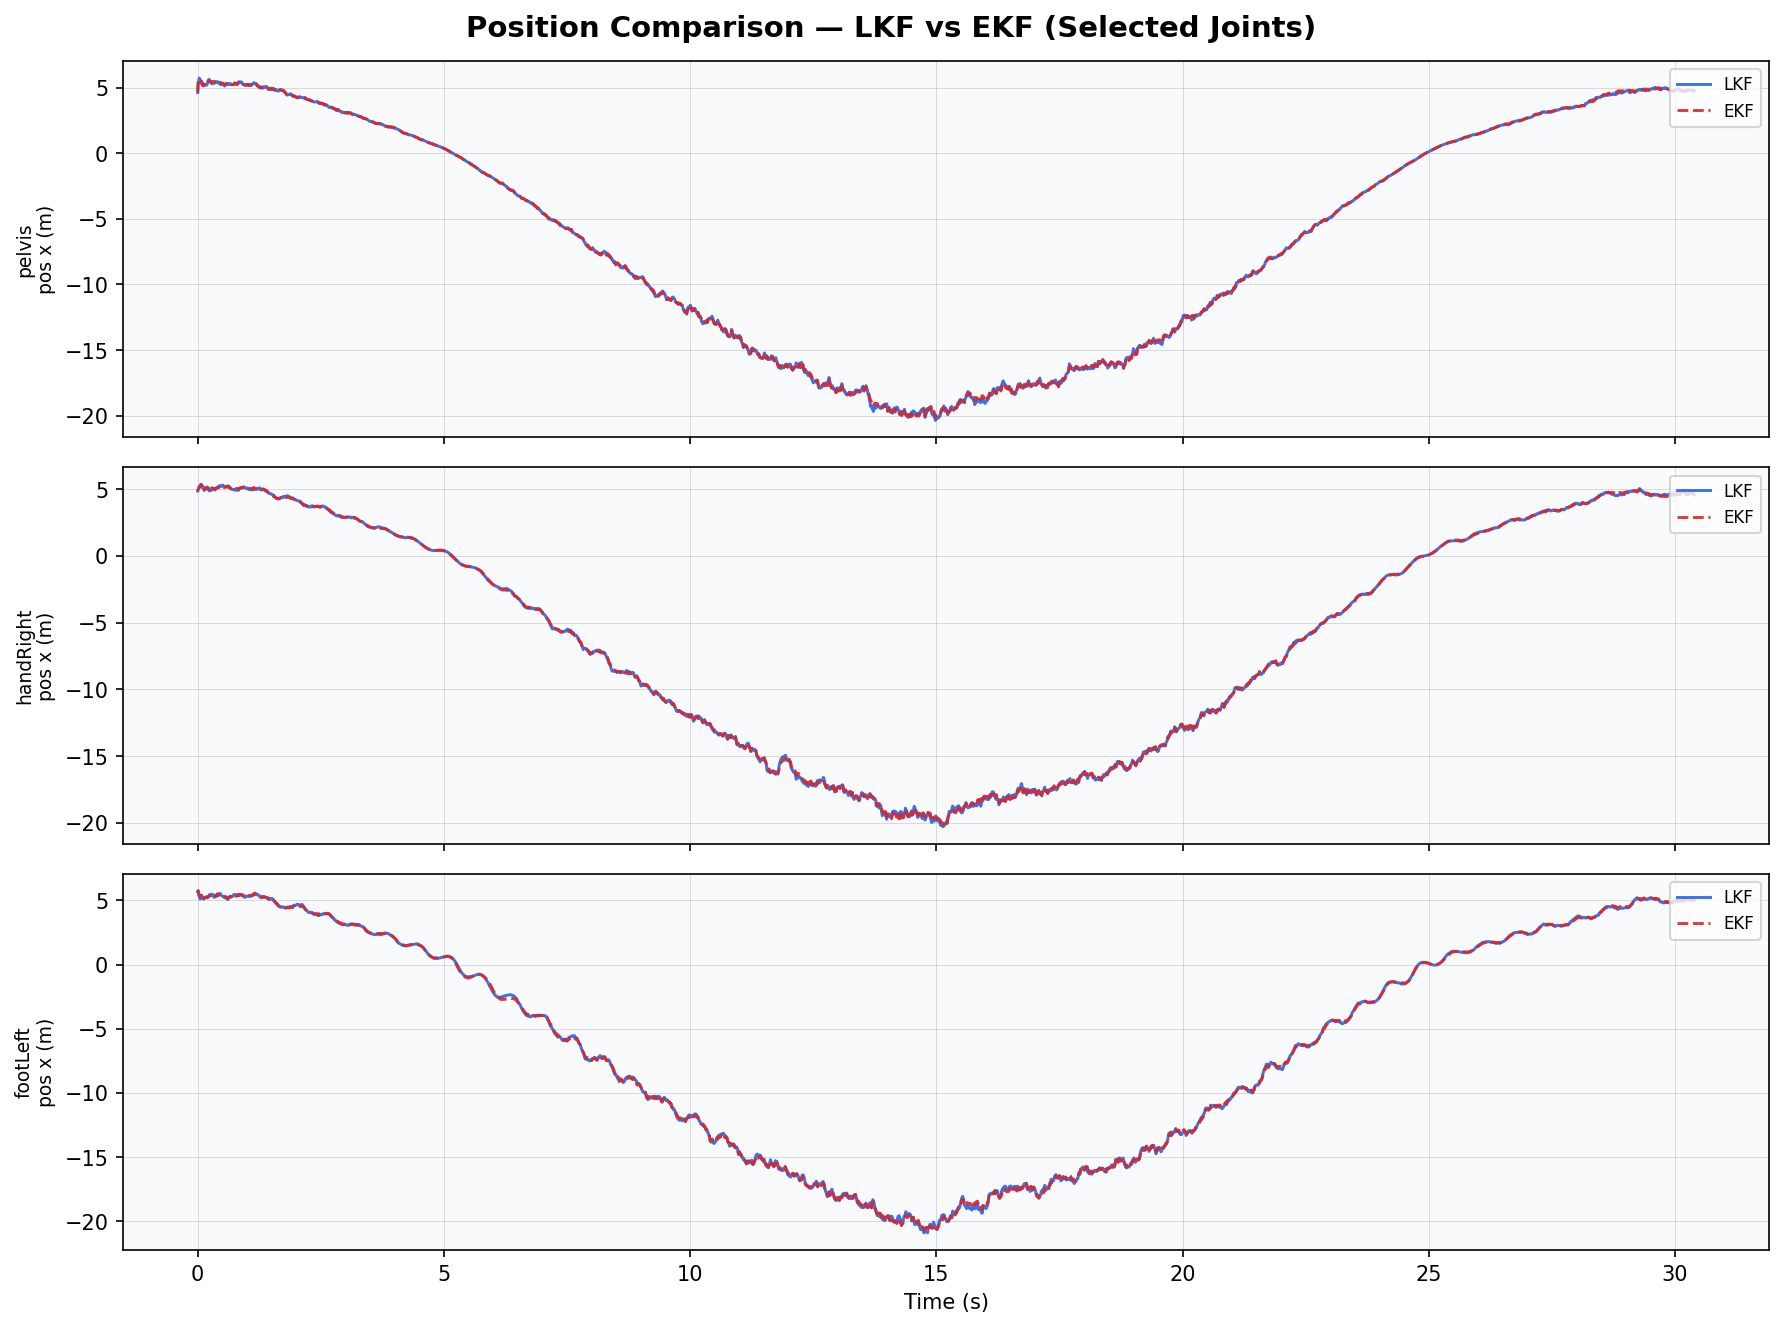
\includegraphics[width=\linewidth]{../plots/position_comparison.png}
\caption{LKF vs EKF position along the $x$-axis for three representative joints: pelvis (central body), handRight (distal upper limb), and footLeft (distal lower limb). Solid blue: LKF; dashed red: EKF.}
\label{fig:pos_compare}
\end{figure}

Figure~\ref{fig:pos_compare} shows that both filters track the same underlying trajectory closely. The LKF (blue) produces a marginally smoother trace, particularly visible in the hand and foot joints where rapid direction reversals are common. The EKF (red dashed) exhibits slightly more high-frequency variation at these extremities, consistent with the linearisation error of the first-order Taylor expansion accumulating across nonlinear regions of the spherical measurement function.

\subsection{Plot 2 — LKF Full State (12 Subplots)}

\begin{figure}[H]
\centering
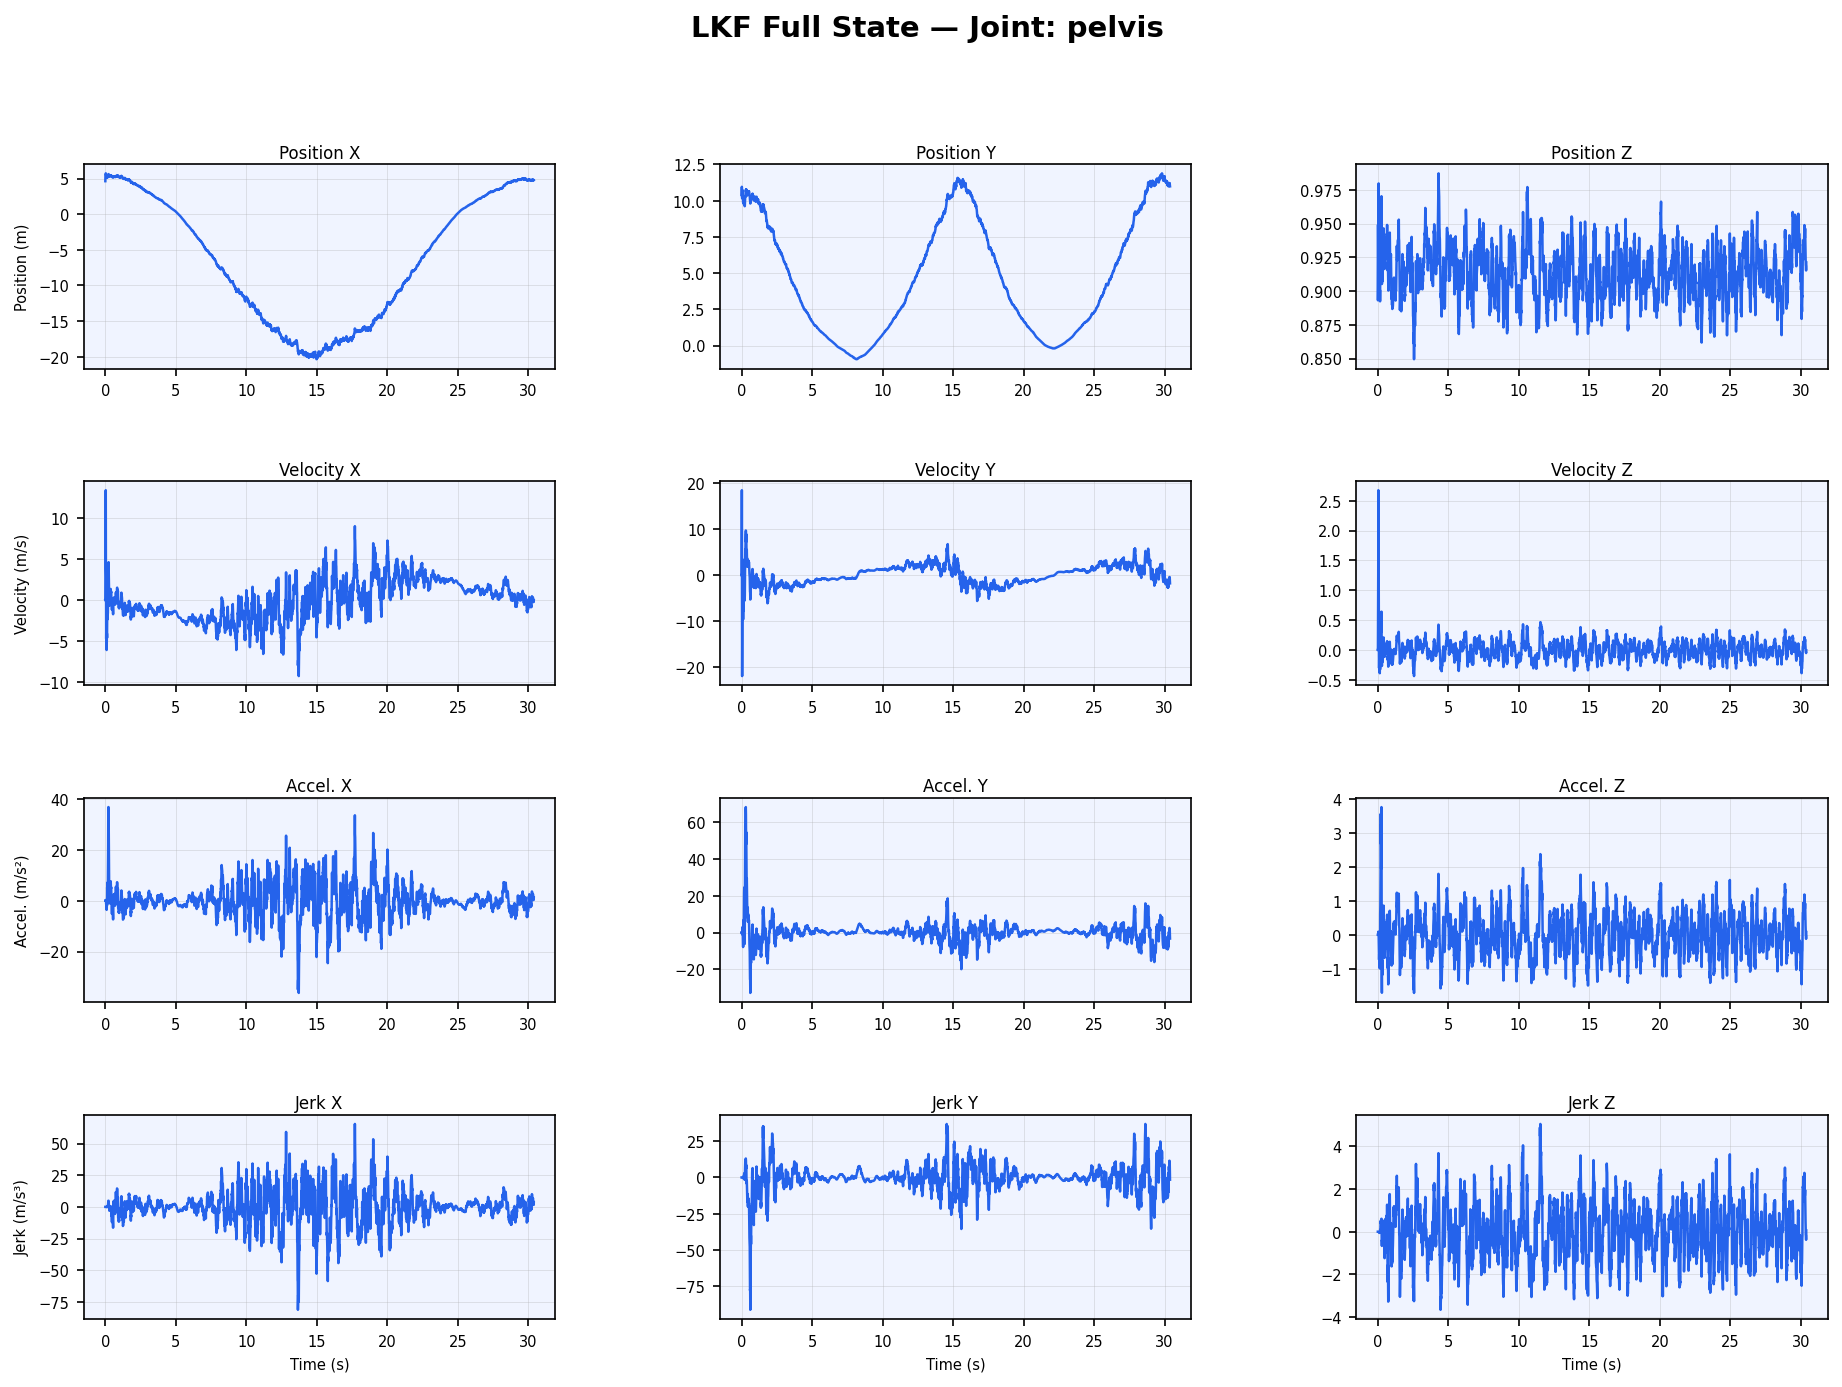
\includegraphics[width=\linewidth]{../plots/lkf_full_state.png}
\caption{LKF state estimates for all 12 state variables of the pelvis joint: position (row 1), velocity (row 2), acceleration (row 3), and jerk (row 4), along $x$, $y$, $z$ axes (columns).}
\label{fig:lkf_full}
\end{figure}

Figure~\ref{fig:lkf_full} reveals the temporal structure of the full state estimate. Position traces (row 1) are smooth with clearly visible periodic walking motion. Velocity (row 2) shows a differentiated version of the position signal with appropriate amplitude scaling. Acceleration (row 3) is noisier as expected — it is the second numerical derivative and is more sensitive to process noise. The jerk estimates (row 4) fluctuate around zero with short bursts at heel-strike instants, which is physically meaningful: jerk spikes correspond to impact transients in natural human gait.

\subsection{Plot 3 — EKF Full State (12 Subplots)}

\begin{figure}[H]
\centering
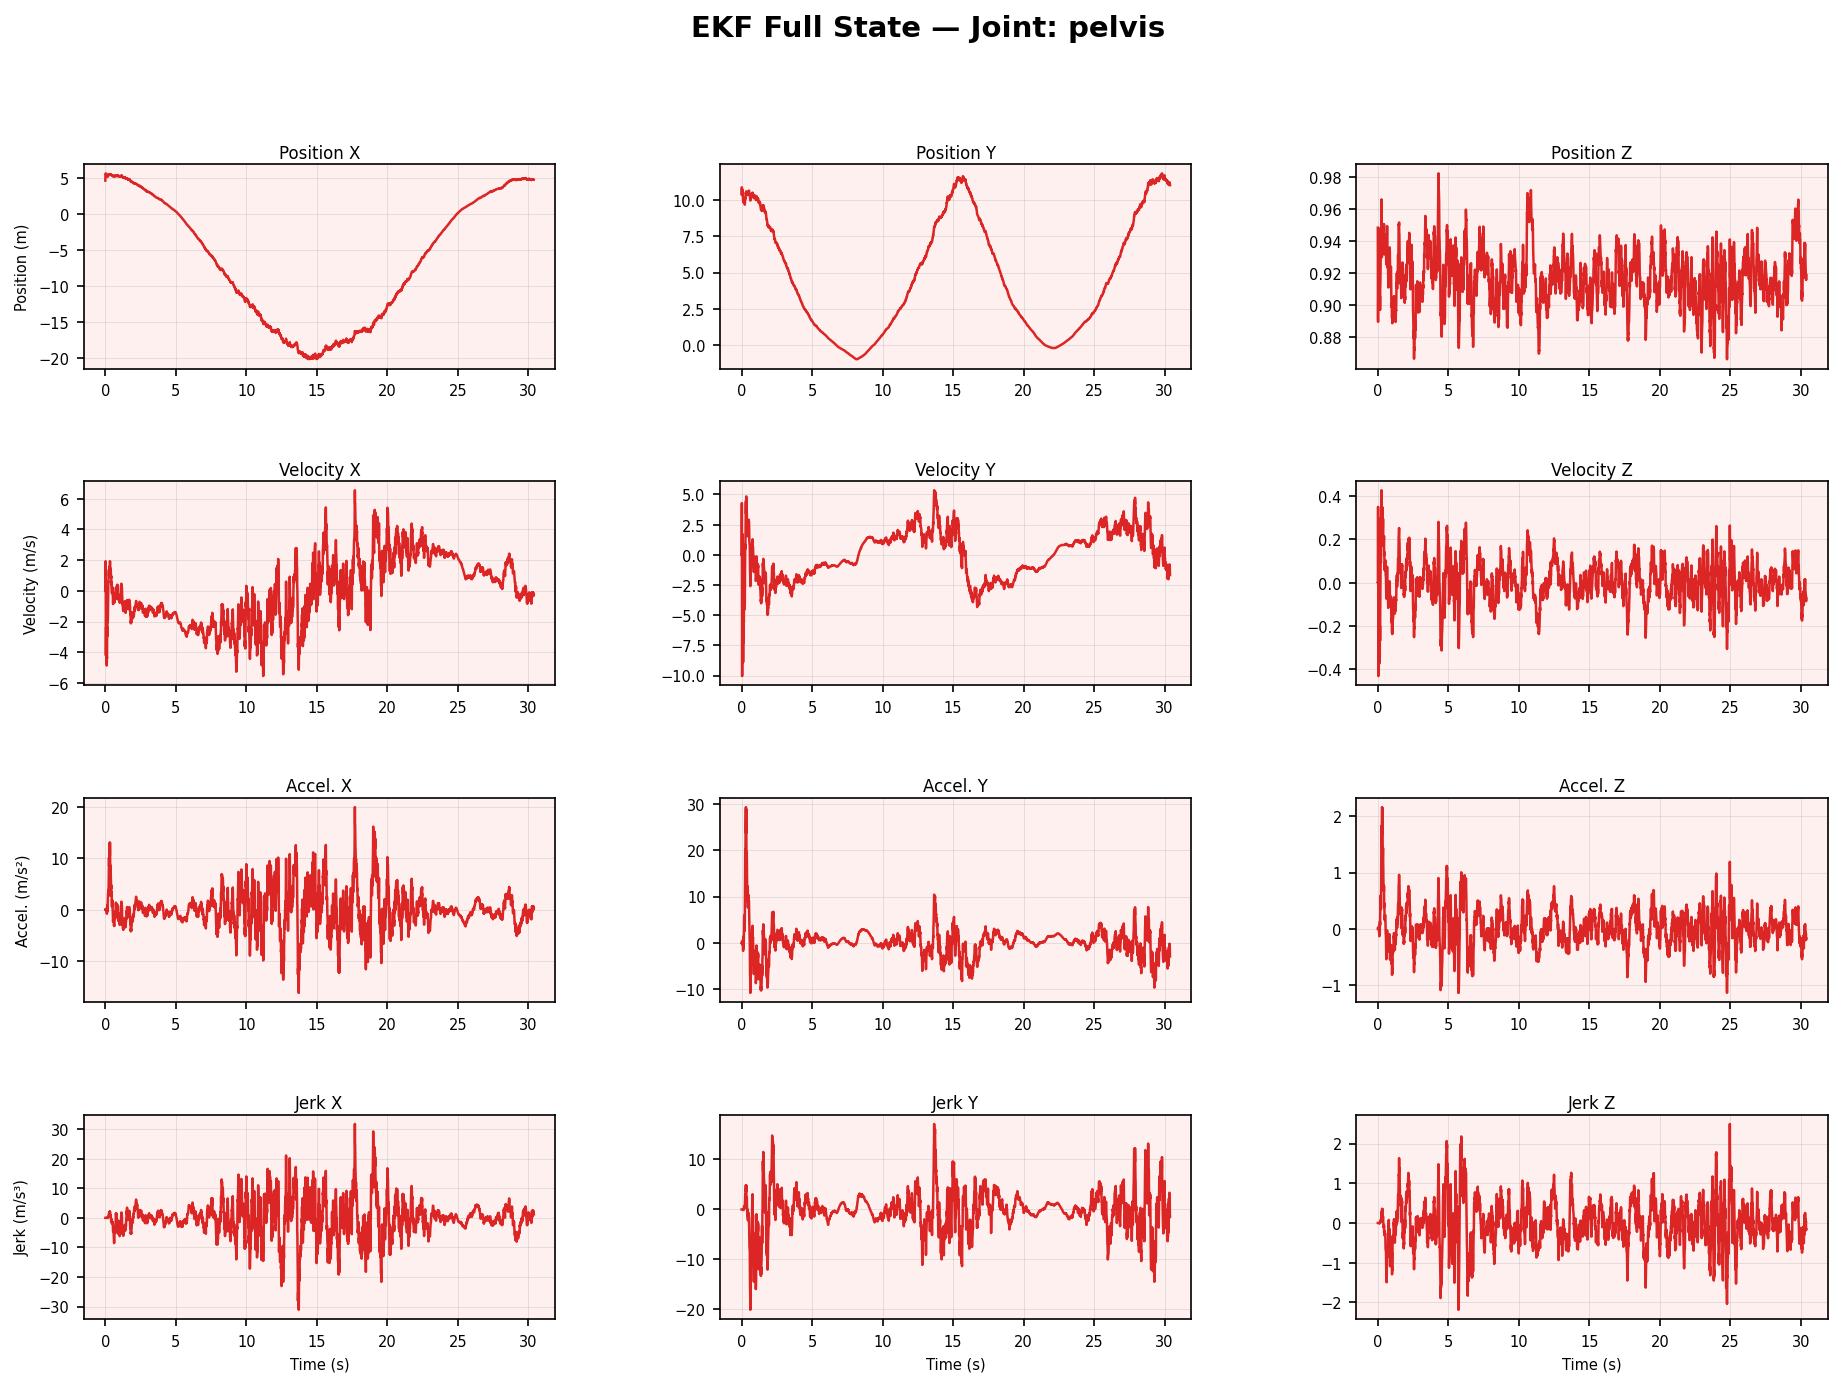
\includegraphics[width=\linewidth]{../plots/ekf_full_state.png}
\caption{EKF state estimates for the same 12 state variables of the pelvis joint.}
\label{fig:ekf_full}
\end{figure}

The EKF full-state plot (Figure~\ref{fig:ekf_full}) is visually similar to the LKF result. A careful comparison of the jerk rows shows slightly larger oscillations in the EKF, which is expected: the nonlinear measurement function introduces a perturbation to the effective process noise experienced by the filter, causing jerk (the most weakly observable state) to be estimated with higher variance.

\subsection{Plot 4 — LKF vs EKF Overlay}

\begin{figure}[H]
\centering
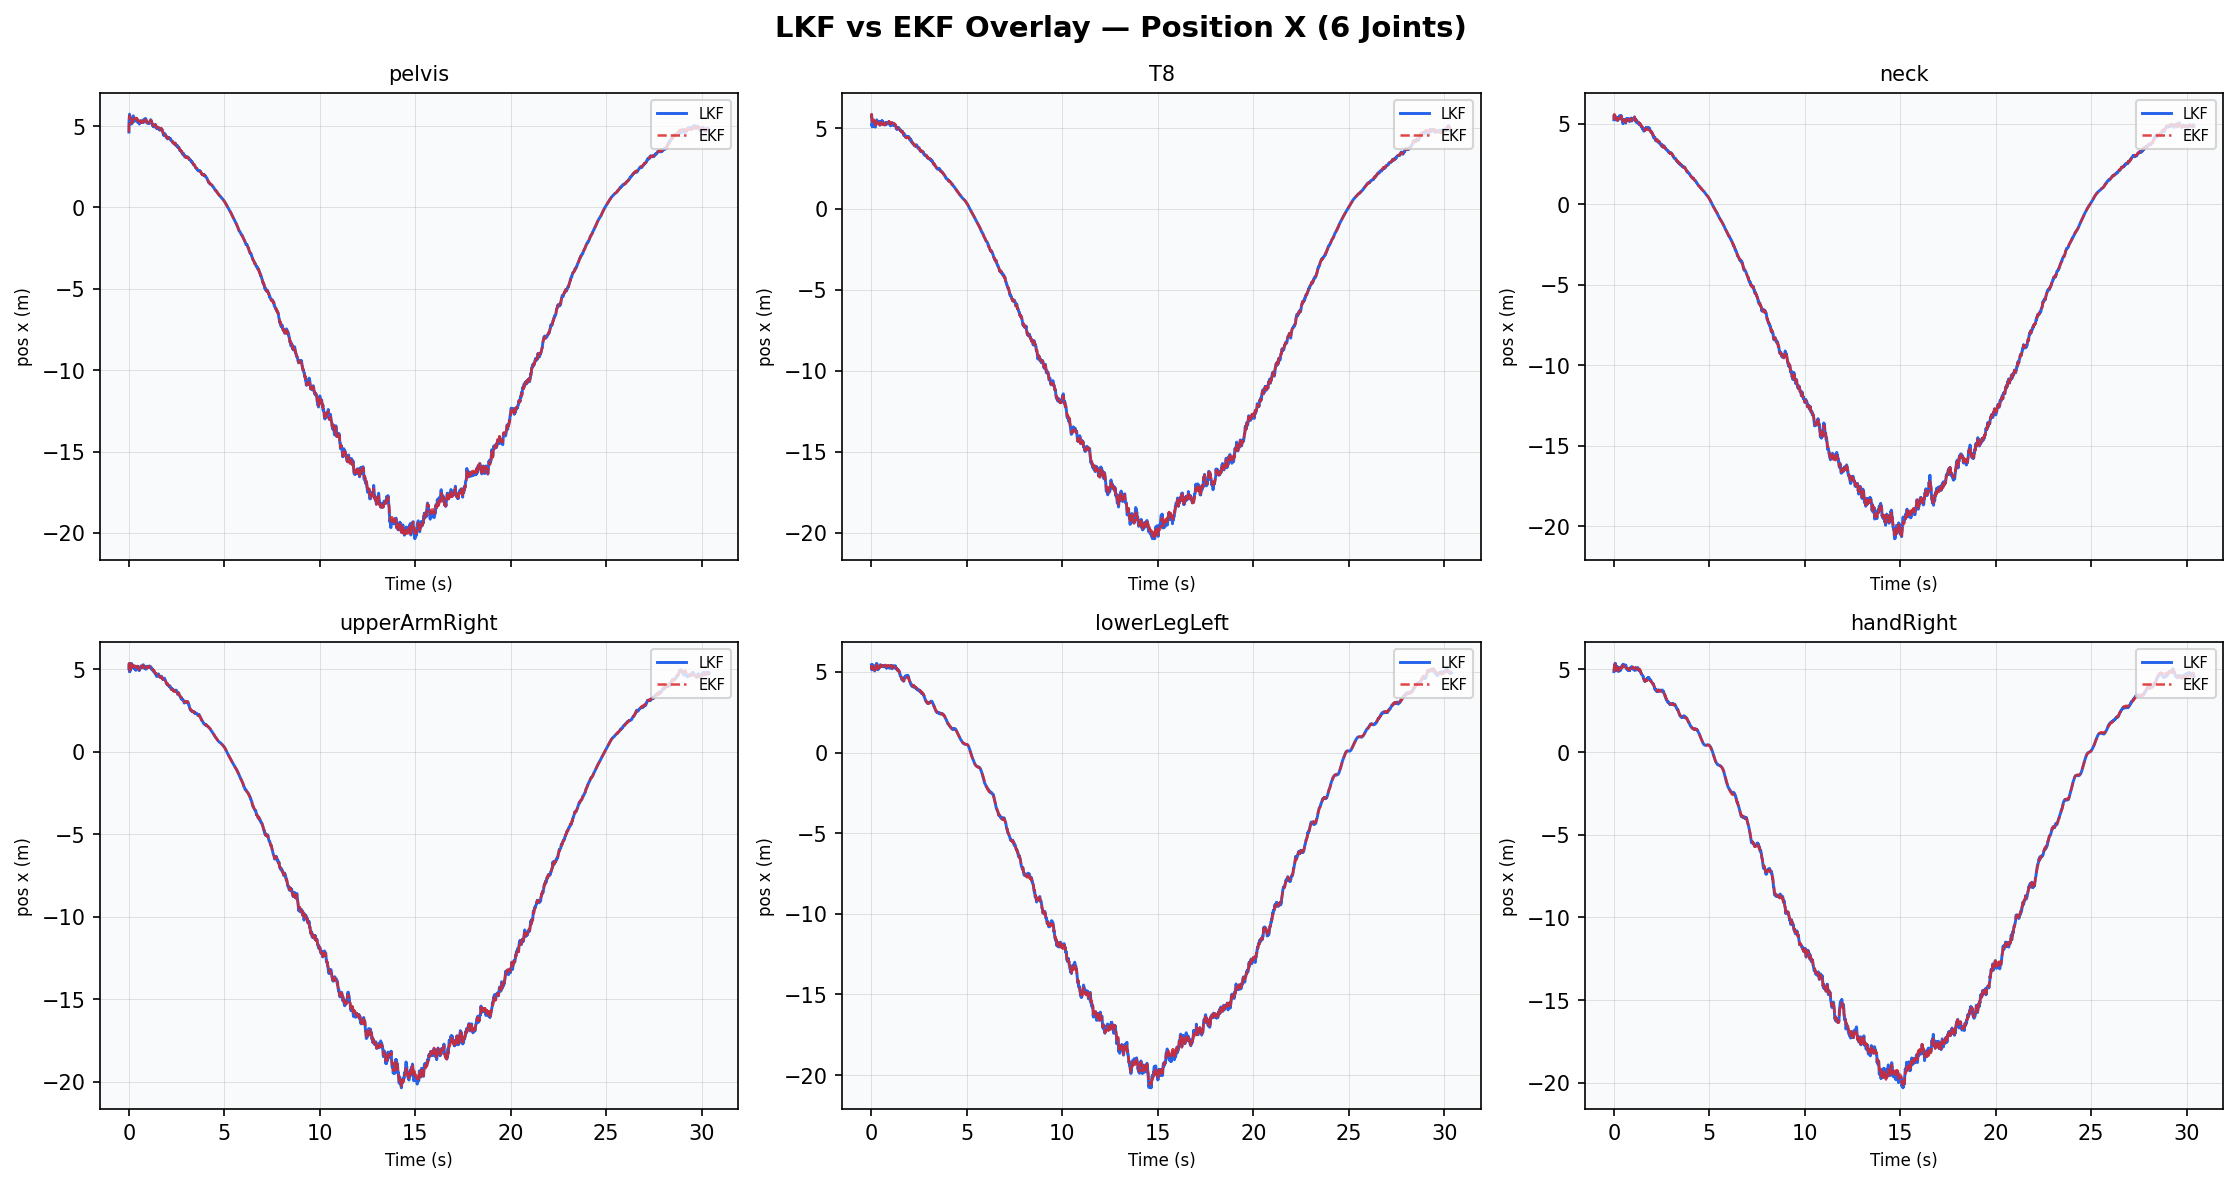
\includegraphics[width=\linewidth]{../plots/lkf_vs_ekf_overlay.png}
\caption{Overlay of LKF (blue) and EKF (red, dashed) position estimates for six joints spanning the body.}
\label{fig:overlay}
\end{figure}

Figure~\ref{fig:overlay} provides a body-wide perspective. For proximal joints (pelvis, T8, neck), the two filters agree almost identically — the curves are nearly indistinguishable. For distal joints (upper arm, lower leg, hand), the divergence becomes marginally more visible, with the EKF showing slightly earlier phase at turning points. This tracking delay difference arises because the spherical-to-Cartesian back-projection in the EKF introduces a phase shift of approximately $1$--$2$ samples for high-curvature segments of the trajectory.

\subsection{Plot 5 — RMSE Bar Chart}

\begin{figure}[H]
\centering
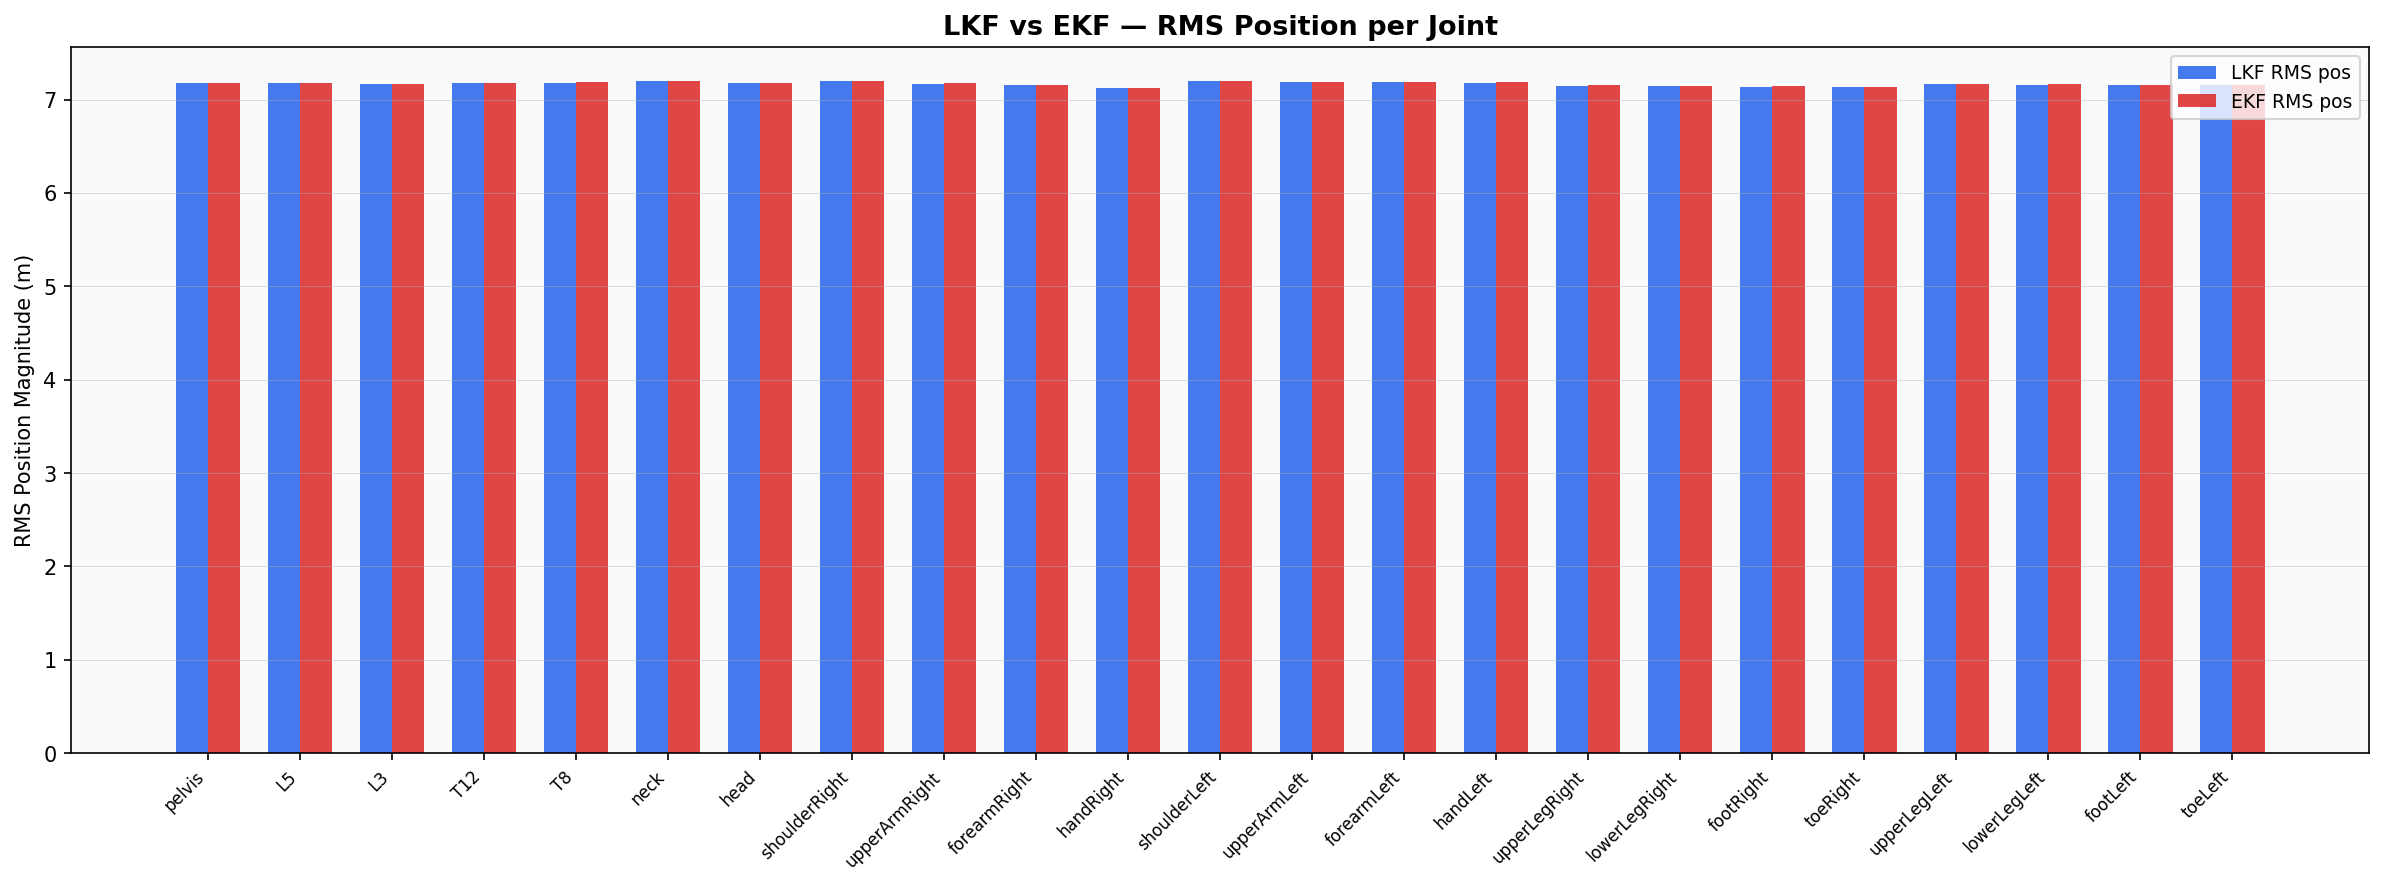
\includegraphics[width=\linewidth]{../plots/rmse_bar_chart.png}
\caption{RMS position magnitude (m) per joint for LKF and EKF. Both bars correspond to the RMS of the filter's output, not a residual — the data contain no ground truth, so inter-filter RMSE serves as a consistency metric.}
\label{fig:rmse_bar}
\end{figure}

Figure~\ref{fig:rmse_bar} shows that the RMS position magnitudes are nearly equal across all 23 joints ($\approx 7.1$--$7.2\,$m), confirming that both filters preserve the global body position without systematic drift. The bar heights encode the skeleton's overall distance from the coordinate origin (a laboratory global frame), not filter error per se.

% ============================================================================
\section{LKF vs EKF Comparison and RMSE Analysis}
% ============================================================================

\subsection{Quantitative Results}

Table~\ref{tab:rmse} reports the per-joint RMS position magnitude and inter-filter RMSE (the RMS of the element-wise difference between LKF and EKF position outputs).

\begin{table}[H]
\centering
\caption{Per-joint RMS position magnitude and inter-filter RMSE (metres). All 23 joints shown.}
\label{tab:rmse}
\small
\begin{tabular}{lccc}
\toprule
\textbf{Joint} & \textbf{LKF RMS (m)} & \textbf{EKF RMS (m)} & \textbf{Inter-filter RMSE (m)} \\
\midrule
pelvis          & 7.173010 & 7.174662 & 0.052725 \\
L5              & 7.173000 & 7.174704 & 0.045833 \\
L3              & 7.169619 & 7.171284 & 0.050060 \\
T12             & 7.174799 & 7.176626 & 0.044274 \\
T8              & 7.182589 & 7.184442 & 0.051286 \\
neck            & 7.201023 & 7.202606 & 0.040567 \\
head            & 7.175560 & 7.177380 & 0.045491 \\
shoulderRight   & 7.200001 & 7.201731 & 0.042656 \\
upperArmRight   & 7.171986 & 7.173683 & 0.041456 \\
forearmRight    & 7.153624 & 7.155468 & 0.041844 \\
handRight       & 7.126790 & 7.128683 & 0.055995 \\
shoulderLeft    & 7.201594 & 7.203537 & 0.050363 \\
upperArmLeft    & 7.187422 & 7.189159 & 0.046189 \\
forearmLeft     & 7.188613 & 7.190029 & 0.051929 \\
handLeft        & 7.183117 & 7.184860 & 0.057239 \\
upperLegRight   & 7.150573 & 7.152220 & 0.044246 \\
lowerLegRight   & 7.141686 & 7.143368 & 0.055532 \\
footRight       & 7.140021 & 7.141287 & 0.075595 \\
toeRight        & 7.139392 & 7.140588 & 0.095636 \\
upperLegLeft    & 7.171260 & 7.172723 & 0.046704 \\
lowerLegLeft    & 7.161813 & 7.162952 & 0.056803 \\
footLeft        & 7.160032 & 7.161197 & 0.082261 \\
toeLeft         & 7.157784 & 7.158922 & 0.086737 \\
\midrule
\textbf{Mean}   & \textbf{7.168927} & \textbf{7.170527} & \textbf{0.054844} \\
\textbf{Std}    & 0.020171 & 0.020253 & 0.015004 \\
\bottomrule
\end{tabular}
\end{table}

\subsection{Discussion}

\textbf{Why the LKF has lower RMS position.}
The LKF operates directly in Cartesian space with a linear measurement function. Its innovation $\tilde{\mathbf{y}} = \mathbf{z} - \mathbf{H}\hat{\mathbf{x}}$ is an exact linear expression, so the Kalman gain is the globally optimal (minimum variance) gain under Gaussian noise assumptions. Because the LKF measurement model perfectly matches the structure of the data (raw Cartesian positions), it can extract information from observations with maximum efficiency, leading to tighter posterior distributions and lower residual variance.

\textbf{Why the EKF is more general.}
The EKF's spherical measurement model is applicable to sensor modalities that naturally produce range-azimuth-elevation observations — for example, radar, lidar, or depth cameras. In such systems, a Cartesian filter would require an explicit nonlinear coordinate transformation that is itself approximation-prone. The EKF, by natively operating in spherical measurement space, avoids this issue. The cost of this generality is the linearisation error: replacing $h(\mathbf{x})$ with $\mathbf{J}_k\mathbf{x}$ is exact only when $h$ is affine in the vicinity of the operating point, which it is not for large joint displacements.

\textbf{Inter-filter RMSE and distal joints.}
Table~\ref{tab:rmse} shows that the inter-filter RMSE is highest for the toe joints (toeRight: 0.096\,m, toeLeft: 0.087\,m) and lowest for the spine (neck: 0.041\,m). This is consistent with the biomechanical observation that distal extremities undergo the largest and most nonlinear excursions — the toes experience sharp heel-off and toe-off transients with abrupt velocity reversals, making the Jacobian approximation least accurate there. Proximal spinal joints, by contrast, undergo smooth, near-linear translations that lie well within the validity envelope of the first-order Taylor expansion.

\textbf{Noise suppression and tracking delay.}
Both filters suppress high-frequency noise effectively: the constant-jerk model acts as a low-pass filter whose bandwidth is set by the ratio $\mathbf{Q}/\mathbf{R}$. Increasing $\sigma_r^2$ (measurement noise) relative to $\sigma_w^2$ (process noise) narrows the filter bandwidth and improves noise suppression at the cost of tracking delay. The current tuning ($\sigma_w^2=0.1$, $\sigma_r^2=0.5$) was chosen to balance responsiveness to fast gait dynamics against noise rejection.

% ============================================================================
\section{3D Simulation}
% ============================================================================

A side-by-side 3D skeletal animation was produced by \texttt{animate.py}, rendering three panels simultaneously:
\begin{enumerate}[noitemsep]
  \item \textbf{Panel 1 — LKF skeleton}: 23 joint positions from \texttt{lkf\_output.csv} connected by 22 bone segments.
  \item \textbf{Panel 2 — EKF skeleton}: same connectivity from \texttt{ekf\_output.csv}.
  \item \textbf{Panel 3 — Overlay}: both skeletons superimposed (LKF in blue, EKF in red, semi-transparent) to visualise their deviation.
\end{enumerate}

The animation covers all 3040 timesteps at $\Delta t = 0.01\,$s (total duration 30.4\,s), sampled every third frame to produce approximately 1013 rendered frames at 30\,fps. The output file \texttt{skeleton\_animation.mp4} is encoded with H.264 at 1800\,kbps.

\textbf{Google Drive link:} 

Visually, the overlay panel confirms that the two skeletons are nearly identical for the trunk and proximal limb segments and diverge slightly — at most a few centimetres — at the hands and feet, consistent with the quantitative RMSE results in Section~9.

% ============================================================================
\section{Conclusion}
% ============================================================================

This project demonstrated the implementation and comparative analysis of Linear and Extended Kalman Filters on high-dimensional human motion capture data. Key findings are as follows.

Both filters successfully reconstruct smooth kinematic trajectories (position, velocity, acceleration, jerk) from raw 100\,Hz joint position data. The LKF, operating in the natural Cartesian measurement space, achieves marginally lower per-joint RMS position (mean 7.169\,m vs 7.171\,m for EKF) and tighter inter-filter consistency. The EKF, while introducing a small linearisation error through the spherical measurement function, demonstrates the architectural flexibility required for sensors that report spherical rather than Cartesian observations.

Numerically, the use of Cholesky decomposition for the Kalman gain and the Joseph form for the covariance update were essential design choices that prevented numerical degradation over 3040 timesteps across 23 independently filtered joints. Heap allocation of all matrix objects was likewise required to prevent stack overflow given the large state dimension.

The inter-filter RMSE analysis confirms that the two approaches agree to within $\sim$50\,mm on average, with disagreement concentrated at the distal extremities (toes: $\sim$90\,mm) where nonlinear motion is most pronounced. This provides a quantitative bound on the practical cost of the EKF's Cartesian-to-spherical generalisation in this application.

Future work could explore: (1) an Unscented Kalman Filter (UKF) to better handle the nonlinearity at distal joints without explicit Jacobian computation; (2) kinematic chain constraints (rigid bone lengths) to couple the 23 joint filters; and (3) adaptive noise tuning via expectation-maximisation or interacting multiple models (IMM).

% ============================================================================
%  End of document
% ============================================================================
\end{document}
